% --- Template for thesis / report with tktltiki2 class ---
% 
% last updated 2013/02/15 for tkltiki2 v1.02

\documentclass[finnish, grading]{tktltiki2}

% tktltiki2 automatically loads babel, so you can simply
% give the language parameter (e.g. finnish, swedish, english, british) as
% a parameter for the class: \documentclass[finnish]{tktltiki2}.
% The information on title and abstract is generated automatically depending on
% the language, see below if you need to change any of these manually.
% 
% Class options:
% - grading                 -- Print labels for grading information on the front page.
% - disablelastpagecounter  -- Disables the automatic generation of page number information
%                              in the abstract. See also \numberofpagesinformation{} command below.
%
% The class also respects the following options of article class:
%   10pt, 11pt, 12pt, final, draft, oneside, twoside,
%   openright, openany, onecolumn, twocolumn, leqno, fleqn
%
% The default font size is 11pt. The paper size used is A4, other sizes are not supported.
%
% rubber: module pdftex

% --- General packages ---

\usepackage[utf8]{inputenc}
\usepackage[T1]{fontenc}
\usepackage{lmodern}
\usepackage{microtype}
\usepackage{amsfonts,amsmath,amssymb,amsthm,booktabs,color,enumitem,graphicx}
\usepackage[pdftex,hidelinks]{hyperref}
\usepackage{multirow}
\usepackage{tabulary}
\usepackage{float}
\usepackage{enumitem}
%\usepackage{paralist}
\usepackage{listings}

\definecolor{dkgreen}{rgb}{0,0.6,0}
\definecolor{gray}{rgb}{0.5,0.5,0.5}
\definecolor{mauve}{rgb}{0.58,0,0.82}

\lstset{frame=tb,
  language=Java,
  aboveskip=3mm,
  belowskip=3mm,
  showstringspaces=false,
  columns=flexible,
  basicstyle={\small\ttfamily},
  numbers=none,
  numberstyle=\tiny\color{gray},
  keywordstyle=\color{blue},
  commentstyle=\color{dkgreen},
  stringstyle=\color{mauve},
  breaklines=true,
  breakatwhitespace=true,
  tabsize=3
}

\hyphenation{luok-ka-mu-taa-ti-o-o-pe-raat-to-ri}

% Automatically set the PDF metadata fields
\makeatletter
\AtBeginDocument{\hypersetup{pdftitle = {\@title}, pdfauthor = {\@author}}}
\makeatother

% References ilman bracket

\makeatletter 
\renewcommand\@biblabel[1]{#1} 
\makeatother

% --- Language-related settings ---
%
% these should be modified according to your language

% babelbib for non-english bibliography using bibtex
\usepackage[fixlanguage]{babelbib}
\selectbiblanguage{finnish}

% add bibliography to the table of contents
\usepackage[nottoc]{tocbibind}
% tocbibind renames the bibliography, use the following to change it back
\settocbibname{Lähteet}

% --- Theorem environment definitions ---

\newtheorem{lau}{Lause}
\newtheorem{lem}[lau]{Lemma}
\newtheorem{kor}[lau]{Korollaari}

\theoremstyle{definition}
\newtheorem{maar}[lau]{Määritelmä}
\newtheorem{ong}{Ongelma}
\newtheorem{alg}[lau]{Algoritmi}
\newtheorem{esim}[lau]{Esimerkki}

\theoremstyle{remark}
\newtheorem*{huom}{Huomautus}


% --- tktltiki2 options ---
%
% The following commands define the information used to generate title and
% abstract pages. The following entries should be always specified:

\title{Ohjelmistoarkkitehtuurien harjoitustyö}
\author{Eveliina Pakarinen}
\date{\today}
\level{Harjoitustyö}
\abstract{}

% The following can be used to specify keywords and classification of the paper:

\keywords{testaus, testit, mutaatiotestaus, oliojärjestelmät, testien laatu}

% classification according to ACM Computing Classification System (http://www.acm.org/about/class/)
% This is probably mostly relevant for computer scientists
% uncomment the following; contents of \classification will be printed under the abstract with a title
% "ACM Computing Classification System (CCS):"
% \classification{D.2.4 [Software/Program Verification]
%\\D.2.5 [Testing and Debugging]
%\\D.3.3 [Language Constructs and Features]}

% If the automatic page number counting is not working as desired in your case,
% uncomment the following to manually set the number of pages displayed in the abstract page:
%
% \numberofpagesinformation{16 sivua + 10 sivua liitteissä}
%
% If you are not a computer scientist, you will want to uncomment the following by hand and specify
% your department, faculty and subject by hand:
%
% \faculty{Matemaattis-luonnontieteellinen}
% \department{Tietojenkäsittelytieteen laitos}
% \subject{Tietojenkäsittelytiede}
%
% If you are not from the University of Helsinki, then you will most likely want to set these also:
%
% \university{Helsingin Yliopisto}
% \universitylong{HELSINGIN YLIOPISTO --- HELSINGFORS UNIVERSITET --- UNIVERSITY OF HELSINKI} % displayed on the top of the abstract page
% \city{Helsinki}
%


\begin{document}

% --- Front matter ---

\frontmatter      % roman page numbering for front matter

\maketitle        % title page
%\makeabstract     % abstract page

\tableofcontents  % table of contents

% --- Main matter ---

\mainmatter       % clear page, start arabic page numbering

% Write some science here.

% Tähän tekstiä. \\ Esimerkki lähdeviitteestä: ~\cite{toinen}.

%\[\frac{a}{b}\]

\section{Johdanto}

Perinteisiä ohjelmistojen testausmenetelmiä on olioperustaisen ohjelmoinnin kehityksen myötä sopeutettu uusiin olio-ohjelmoinnin mukana tuleviin haasteisiin. Olio-ohjelmoinnin avulla voidaan ratkaista joitakin proseduraalisen ohjelmoinnin ongelmia~\cite[s. 86]{Mariani:Pezze:2008}. O\-li\-o-oh\-jel\-moin\-nin piirteet, kuten kapselointi ja perintä, aiheuttavat kuitenkin uusia ongelmia, jotka vaativat uusien testaus- ja analysointimenetelmien kehittämistä.



\section{Testaus oliojärjestelmissä}

Olioperustaisen ohjelmoinnin kehityksen myötä klassisia ohjelmistojen testausmenetelmiä on sopeutettu mahdollistamaan \textit{oliojärjestelmien} (\textit{object oriented systems}) kattava ja laadukas testaaminen. Vaikka olioperustainen ohjelmointi ratkaisee joitakin proseduraalisen ohjelmoinnin suunnittelu- ja toteutusongelmia, olio-ohjelmoinnin mukana tulevat uudet haasteet vaativat uusien testaus- ja analysointimenetelmien kehittämistä~\cite[s. 86]{Mariani:Pezze:2008}. 

\subsection{Testauksen rooli}

IEEE:n standardin mukaan \textit{ohjelmointivirheen} (\textit{error}) aiheuttamaa ohjelmiston lähdekoodiin päässyttä virheellistä kohtaa kutsutaan \textit{viaksi} (\textit{fault})~\cite[s. 5]{IEEE:2009}. Lähdekoodissa oleva vika saattaa ohjelman suoritusaikana ilmetä \textit{virheenä} (\textit{failure})~\cite[s. 5]{IEEE:2009}. Virhe ilmenee, kun ohjelma ei suorituksen aikana toimi odotetulla tavalla.

Testausta käytetään ohjelmistokehityksessä ohjelmiston laadun varmistamiseen ja auttamaan lähdekoodissa esiintyvien vikojen havaitsemisessa jo kehitysvaiheen aikana. Ohjelmistojen testaamisen ensisijainen tavoite on siis paljastaa vikoja, joiden havaitseminen muiden laadunvarmistusmenetelmien avulla olisi työlästä tai mahdotonta~\cite[s. 59]{Binder:1999}. Testauksen avulla pyritään myös varmistamaan, että ohjelma toimii sille asetettujen vaatimusten mukaisesti. %\textit{\textbf{The primary role of software testing is to reveal bugs that would be too costly or impossible to find with other verification and validation techniques. A secondary purpose is to show that the system under test complies with its stated requirements for a given test suite.}}

Olio-ohjelmoinnissa testaukseen tuovat haasteita olio-ohjelmien erityispiirteet, joita ovat muun muuassa kapselointi, perintä, dynaaminen sidonta ja polymorfismi~\cite[s. 86]{Mariani:Pezze:2008}.


% \newpage

\section{Mutaatiotestaus}

Testaukseen sisältyvien rajoitusten lisäksi testaukseen liittyy myös epävarmuutta käytettävän testausjärjestelmän oikeellisuudesta ja oikeellisuuden varmistamisesta~\cite[s. 209]{Manna:Waldinger:1978}. Tämä herättää kysymyksen siitä, kuka voi ''valvoa valvojia'' eli kuinka varmistetaan ohjelmiston testien laadukkuus. Yksi menetelmä testien laadun selvittämiseen on \textit{mutaatiotestaus}. Mutaatiotestauksen avulla voidaan mitata, kuinka tehokkaasti ohjelmiston testeillä havaitaan ohjelmistossa esiintyviä vikoja~\cite[s. 649]{Jia:Harman:2011}.

\subsection{Historia ja teoreettinen perusta}

Mutaatiotestauksesta kirjoitettiin ensimmäistä kertaa jo 1970-luvulla. Richard DeMillon, Richard Liptonin ja Frederick Saywardin artikkeli ''\textit{Hints on Test Data Selection: Help for the Practicing Programmer}''~\cite{DeMillo:Lipton:Sayward:1978} vuodelta 1978 on yksi ensimmäisistä uraauurtavista mutaatiotestausta esittelevistä artikkeleista. Mutaatiotestauksen tutkimus on lisääntynyt vuosien kuluessa, ja erityisesti 2000-luvulla uusia tutkimuksia ja tuloksia on julkaistu paljon~\cite[s. 1102]{Offutt:2011}. Tutkimuksessa suuntana on ollut etsiä keinoja, joilla mutaatiotestaus voidaan muuttaa käytännölliseksi testausmenetelmäksi~\cite[s. 649]{Jia:Harman:2011}. 

Jefferson Offutt määritteli artikkelissaan yksinkertaiset ja monimutkaiset viat seuraavasti~\cite[s. 6]{Offutt:1992:Coupling}:
\begin{itemize}
  \item Lähdekoodissa olevan \textit{yksinkertaisen vian} voi korjata tekemällä yksittäisen muutoksen lähdekoodin lauseeseen.
  \item \textit{Monimutkaista vikaa} ei voi korjata tekemällä yksittäistä muutosta lähdekoodin lauseeseen.
\end{itemize}

\subsection{Perinteinen mutaatiotestausprosessi}

Perinteisen mutaatiotestausprosessin syötteinä käytetään alkuperäistä ohjelmistoa ja ohjelmistoa testaavia testejä. Mutaatiotestausprosessin aikana olemassa olevien testien laatua kehitetään vaiheittain. Perinteisen mutaatiotestausprosessin työvaiheet on esitelty kuvassa %\ref{figure:Mutaatiotestausprosessi}. Työvaiheet on merkitty kuvaan sinisillä laatikoilla. Työvaiheiden aikana käytettäviä resursseja, kuten ohjelmiston lähdekoodia ja testituloksia, kuvataan vihreillä ja keltaisilla laatikoilla.

%\begin{figure}[H]
%	\centering
%		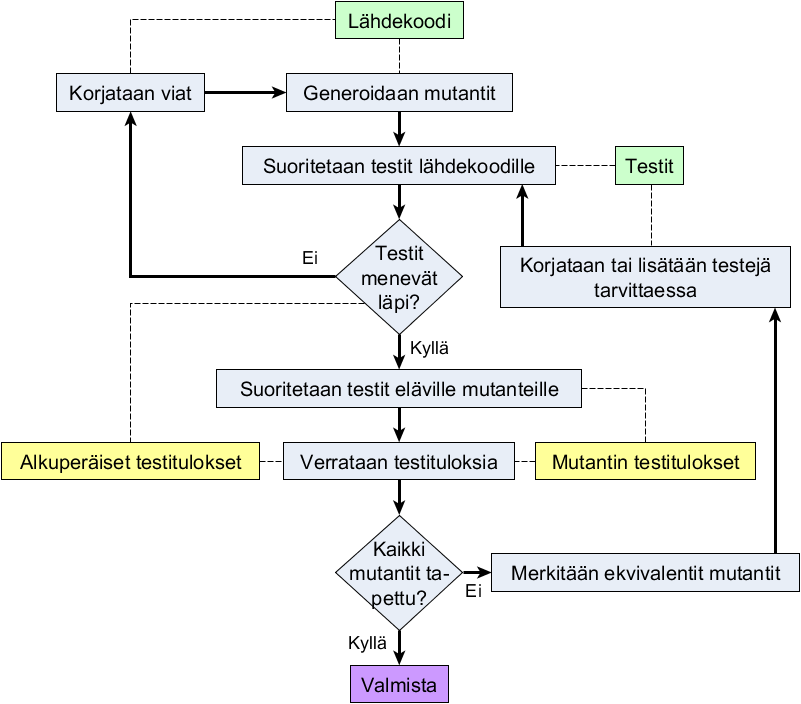
\includegraphics[width=\textwidth]{mutaatiotestausprosessi3}
%	\caption{Perinteinen mutaatiotestausprosessi.}
%	\label{figure:Mutaatiotestausprosessi}
%\end{figure}

Perinteisessä mutaatiotestausprosessissa ensimmäinen työvaihe on käsitellä ohjelmiston alkuperäistä lähdekoodia \textit{mutaatio-operaattoreilla}, jotka muuntavat koodia muodostaen siitä viallisia versioita~\cite[s. 869]{Ma:Harrold:Kwon:2006}. Näitä viallisia ohjelmakoodin versioita kutsutaan mutanteiksi. Mutaatio-operaattorit kuvaavat algoritmeja, joiden avulla lähdekoodia käsitellään koodin muuntamisen aikana~\cite[s. 35]{Offutt:Untch:2001}.


Testien suorituksen jälkeen alkuperäiselle lähdekoodille ja mutanteille suoritettujen testien tuloksia verrataan toisiinsa. Testituloksia verrattaessa voidaan päästä kahteen lopputulokseen~\cite[s. 36]{DeMillo:Lipton:Sayward:1978}. Alkuperäiselle muuntamattomalle lähdekoodille suoritettujen testien tulos voi: 
\begin{enumerate}
  \item erota yhdelle mutantille suoritettujen testien tuloksesta tai
  \item olla sama kuin yhdelle mutantille suoritettujen testien tulos.
\end{enumerate}


\begin{esim}
\vspace{1\baselineskip}\noindent
\begin{lstlisting} 
public class Kauppa {
	private String osoite;
	public void setOsoite(String uusiOsoite){
		this.osoite = uusiOsoite;
	};
	public String getOsoite(){
		return this.osoite;
	};
};

public class Elainkauppa extends Kauppa {
	private String osoite; //IHI-operaattorin lisaama peittava kentta
	private String erikoisala = "kissanruuat";
	public String toString(){
		return "Liikkeen osoite on " + getOsoite() +
		        " ja sen erikoisalana on " + this.erikoisala;
	};
};
\end{lstlisting}
\label{esim:IHIEkvivalenttiMutantti}
\end{esim}

\vspace{1\baselineskip}On todistettu, että ekvivalenttien mutanttien tunnistaminen algoritmisesti yleisessä tapauksessa on ratkaisematon ongelma~\cite[s. 79]{Offutt:Ma:Kwon:2006:MuClassLevel}. Ongelma on kuitenkin herättänyt runsaasti teoreettista kiinnostusta, ja mahdollisia tunnistamistekniikoita on tutkittu paljon~\cite[s. 657]{Jia:Harman:2011}. Ekvivalenttien mutanttien tunnistamiseksi on kehitetty heuristiikkoja, joiden avulla tunnistamisongelma voidaan ratkaista osittain~\cite[s. 79]{Offutt:Ma:Kwon:2006:MuClassLevel}.

\section{Yhteenveto}

Olioperustaisen ohjelmoinnin mukana tulevien uusien haasteiden kohtaaminen vaatii muutoksia ohjelmistojen testausmenetelmiin. Sekä perinteisiä olemassa olevia että uusia testausmenetelmiä kehitetään, jotta olio-ohjelmia voidaan testata kattavasti ja laadukkaasti. 

Perinteisessä ohjelmistotestauksessa keskitytään ohjelmiston toiminnallisuuden testaamiseen ja vikojen etsimiseen ohjelmistosta. Perinteiseen ohjelmistotestaukseen liittyy kuitenkin haasteita ja rajoituksia, jotka aiheuttavat testaukseen epävarmuutta. Yksi haasteista on määrittää, ovatko testauksessa käytettävät testit ja testausjärjestelmä riittävän luotettavia, jotta niiden avulla ohjelmistoa voidaan testata laadukkaasti.

Mutaatiotestaus on vikaperustainen testausmenetelmä, joka tarjoaa ratkaisun testien laadun määrittämiseen liittyvään haasteeseen. Mutaatiotestauksen avulla voidaan mitata ohjelmistoa varten tehtyjen testien kykyä havaita ohjelmistossa esiintyviä vikoja. Mutaatiotestausmenetelmän avulla on siis mahdollista kehittää olemassa olevia testejä ja parantaa testien laatua.

Mutaatiotestauksen käyttö yleisesti osana testausprosessia on kuitenkin vähäistä mutaatiotestaukseen liittyvien haasteiden ja ratkaisemattomien ongelmien takia. Mutaatiotestausta on tutkittu paljon, ja tutkimuksen tavoitteena on ollut etsiä ratkaisuja mutaatiotestaukseen liittyviin ongelmiin. Tutkimuksesta saatujen tietojen pohjalta ongelmiin on kehitetty osittaisia ratkaisuja, joiden avulla mutaatiotestausprosessi on mahdollista automatisoida lähes kokonaan.

Jotta mutaatiotestausmenetelmää voitaisiin tulevaisuudessa hyödyntää aiempaa enemmän tutkimuskäytön ulkopuolella, mutaatiotestauksen käyttöönoton helpottamiseksi olisi kehitettävä automatisoituja mutaatiotestausjärjestelmiä, joissa hyödynnetään mutaatiotestauksen ongelmien ratkaisumenetelmiä. Automatisoitujen mutaatiotestausjärjestelmien avulla mutaatiotestausmenetelmän laaja-alainen käyttö osana ohjelmistokehitystä voisi tulevaisuudessa olla mahdollista.



% --- References ---
%
% bibtex is used to generate the bibliography. The babplain style
% will generate numeric references (e.g. [1]) appropriate for theoretical
% computer science. If you need alphanumeric references (e.g [Tur90]), use
%
\newpage
\bibliographystyle{babalpha-lf}
%
% instead.

%\bibliographystyle{babplain-lf}
\bibliography{references-fi}


% --- Appendices ---

% uncomment the following

% \newpage
% \appendix
% 
% \section{Esimerkkiliite}

\end{document}
